% Created by tikzDevice version 0.12.3.1 on 2021-11-16 18:42:30
% !TEX encoding = UTF-8 Unicode
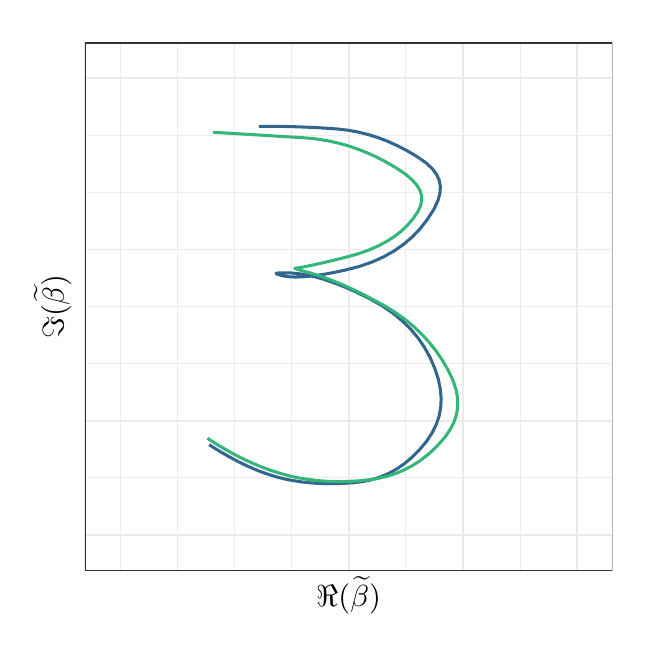
\begin{tikzpicture}[x=1pt,y=1pt]
\definecolor{fillColor}{RGB}{255,255,255}
\path[use as bounding box,fill=fillColor,fill opacity=0.00] (0,0) rectangle (216.81,216.81);
\begin{scope}
\path[clip] (  0.00,  0.00) rectangle (216.81,216.81);
\definecolor{drawColor}{RGB}{255,255,255}
\definecolor{fillColor}{RGB}{255,255,255}

\path[draw=drawColor,line width= 0.6pt,line join=round,line cap=round,fill=fillColor] (  0.00,  0.00) rectangle (216.81,216.81);
\end{scope}
\begin{scope}
\path[clip] ( 20.71, 20.71) rectangle (211.31,211.31);
\definecolor{fillColor}{RGB}{255,255,255}

\path[fill=fillColor] ( 20.71, 20.71) rectangle (211.31,211.31);
\definecolor{drawColor}{gray}{0.92}

\path[draw=drawColor,line width= 0.3pt,line join=round] ( 20.71, 54.13) --
	(211.31, 54.13);

\path[draw=drawColor,line width= 0.3pt,line join=round] ( 20.71, 95.38) --
	(211.31, 95.38);

\path[draw=drawColor,line width= 0.3pt,line join=round] ( 20.71,136.64) --
	(211.31,136.64);

\path[draw=drawColor,line width= 0.3pt,line join=round] ( 20.71,177.89) --
	(211.31,177.89);

\path[draw=drawColor,line width= 0.3pt,line join=round] ( 54.13, 20.71) --
	( 54.13,211.31);

\path[draw=drawColor,line width= 0.3pt,line join=round] ( 95.38, 20.71) --
	( 95.38,211.31);

\path[draw=drawColor,line width= 0.3pt,line join=round] (136.64, 20.71) --
	(136.64,211.31);

\path[draw=drawColor,line width= 0.3pt,line join=round] (177.89, 20.71) --
	(177.89,211.31);

\path[draw=drawColor,line width= 0.6pt,line join=round] ( 20.71, 33.50) --
	(211.31, 33.50);

\path[draw=drawColor,line width= 0.6pt,line join=round] ( 20.71, 74.76) --
	(211.31, 74.76);

\path[draw=drawColor,line width= 0.6pt,line join=round] ( 20.71,116.01) --
	(211.31,116.01);

\path[draw=drawColor,line width= 0.6pt,line join=round] ( 20.71,157.27) --
	(211.31,157.27);

\path[draw=drawColor,line width= 0.6pt,line join=round] ( 20.71,198.52) --
	(211.31,198.52);

\path[draw=drawColor,line width= 0.6pt,line join=round] ( 33.50, 20.71) --
	( 33.50,211.31);

\path[draw=drawColor,line width= 0.6pt,line join=round] ( 74.76, 20.71) --
	( 74.76,211.31);

\path[draw=drawColor,line width= 0.6pt,line join=round] (116.01, 20.71) --
	(116.01,211.31);

\path[draw=drawColor,line width= 0.6pt,line join=round] (157.27, 20.71) --
	(157.27,211.31);

\path[draw=drawColor,line width= 0.6pt,line join=round] (198.52, 20.71) --
	(198.52,211.31);
\definecolor{drawColor}{RGB}{49,103,142}

\path[draw=drawColor,line width= 1.1pt,line join=round] ( 65.56, 66.11) --
	( 69.05, 63.93) --
	( 72.42, 61.97) --
	( 75.65, 60.23) --
	( 78.77, 58.69) --
	( 81.78, 57.35) --
	( 84.68, 56.20) --
	( 87.49, 55.22) --
	( 90.20, 54.40) --
	( 92.82, 53.75) --
	( 95.48, 53.21) --
	( 98.25, 52.77) --
	(101.13, 52.43) --
	(104.13, 52.19) --
	(107.25, 52.06) --
	(110.50, 52.04) --
	(113.90, 52.14) --
	(117.43, 52.36) --
	(120.99, 52.77) --
	(124.33, 53.47) --
	(127.48, 54.46) --
	(130.48, 55.75) --
	(133.37, 57.35) --
	(136.15, 59.27) --
	(138.87, 61.56) --
	(141.53, 64.23) --
	(144.14, 67.34) --
	(146.15, 70.39) --
	(147.64, 73.41) --
	(148.67, 76.44) --
	(149.25, 79.54) --
	(149.41, 82.76) --
	(149.13, 86.18) --
	(148.36, 89.85) --
	(147.06, 93.83) --
	(145.37, 97.72) --
	(143.36,101.34) --
	(141.04,104.71) --
	(138.38,107.88) --
	(135.35,110.86) --
	(131.92,113.68) --
	(128.02,116.34) --
	(123.63,118.85) --
	(118.99,121.13) --
	(114.70,123.03) --
	(110.73,124.59) --
	(107.08,125.84) --
	(103.70,126.80) --
	(100.60,127.49) --
	( 97.74,127.95) --
	( 95.10,128.18) --
	( 92.67,128.22) --
	( 91.12,128.19) --
	( 90.26,128.13) --
	( 89.88,128.07) --
	( 89.79,128.02) --
	( 89.79,127.98) --
	( 89.93,127.88) --
	( 90.40,127.68) --
	( 91.41,127.34) --
	( 92.83,127.01) --
	( 94.58,126.79) --
	( 96.71,126.70) --
	( 99.27,126.77) --
	(102.32,127.03) --
	(105.91,127.50) --
	(110.08,128.23) --
	(114.88,129.25) --
	(119.97,130.57) --
	(124.56,132.17) --
	(128.71,134.04) --
	(132.47,136.16) --
	(135.88,138.55) --
	(139.00,141.22) --
	(141.84,144.20) --
	(144.43,147.51) --
	(146.79,151.21) --
	(148.25,154.35) --
	(148.98,157.03) --
	(149.12,159.39) --
	(148.75,161.54) --
	(147.85,163.61) --
	(146.33,165.70) --
	(144.04,167.88) --
	(140.77,170.17) --
	(137.16,172.31) --
	(133.58,174.17) --
	(130.02,175.77) --
	(126.47,177.12) --
	(122.92,178.22) --
	(119.36,179.10) --
	(115.77,179.75) --
	(112.14,180.18) --
	(108.49,180.44) --
	(104.86,180.66) --
	(101.25,180.84) --
	( 97.66,180.98) --
	( 94.10,181.08) --
	( 90.56,181.13) --
	( 87.03,181.15) --
	( 83.53,181.12) --
	( 83.53,181.12);
\definecolor{drawColor}{RGB}{51,182,122}

\path[draw=drawColor,line width= 1.1pt,line join=round] ( 64.95, 68.43) --
	( 68.50, 66.17) --
	( 71.98, 64.11) --
	( 75.39, 62.25) --
	( 78.74, 60.58) --
	( 82.03, 59.09) --
	( 85.26, 57.78) --
	( 88.44, 56.64) --
	( 91.58, 55.66) --
	( 94.68, 54.83) --
	( 97.81, 54.15) --
	(101.02, 53.60) --
	(104.32, 53.19) --
	(107.71, 52.92) --
	(111.19, 52.79) --
	(114.79, 52.81) --
	(118.50, 52.98) --
	(122.33, 53.31) --
	(126.16, 53.85) --
	(129.76, 54.67) --
	(133.15, 55.77) --
	(136.37, 57.14) --
	(139.44, 58.80) --
	(142.40, 60.77) --
	(145.25, 63.06) --
	(148.02, 65.71) --
	(150.72, 68.75) --
	(152.72, 71.65) --
	(154.12, 74.45) --
	(155.00, 77.22) --
	(155.40, 80.01) --
	(155.35, 82.91) --
	(154.80, 85.98) --
	(153.70, 89.32) --
	(151.98, 92.97) --
	(149.88, 96.59) --
	(147.58, 99.98) --
	(145.05,103.16) --
	(142.30,106.16) --
	(139.30,108.98) --
	(136.04,111.64) --
	(132.49,114.14) --
	(128.62,116.50) --
	(124.61,118.67) --
	(120.83,120.62) --
	(117.28,122.34) --
	(113.95,123.85) --
	(110.82,125.16) --
	(107.89,126.29) --
	(105.15,127.24) --
	(102.58,128.04) --
	(100.19,128.68) --
	( 98.53,129.15) --
	( 97.48,129.49) --
	( 96.88,129.71) --
	( 96.62,129.83) --
	( 96.55,129.88) --
	( 96.55,129.90) --
	( 96.63,129.93) --
	( 96.93,129.95) --
	( 97.49,130.01) --
	( 98.37,130.13) --
	( 99.63,130.35) --
	(101.35,130.69) --
	(103.59,131.16) --
	(106.43,131.80) --
	(109.94,132.62) --
	(114.19,133.65) --
	(118.79,134.89) --
	(122.89,136.30) --
	(126.52,137.86) --
	(129.73,139.56) --
	(132.58,141.39) --
	(135.09,143.37) --
	(137.30,145.50) --
	(139.25,147.79) --
	(140.96,150.27) --
	(141.95,152.41) --
	(142.38,154.31) --
	(142.33,156.08) --
	(141.83,157.83) --
	(140.80,159.66) --
	(139.10,161.65) --
	(136.56,163.84) --
	(132.97,166.27) --
	(128.98,168.56) --
	(124.99,170.57) --
	(121.00,172.29) --
	(116.98,173.74) --
	(112.92,174.93) --
	(108.82,175.87) --
	(104.64,176.55) --
	(100.38,176.99) --
	( 96.07,177.25) --
	( 91.80,177.51) --
	( 87.57,177.77) --
	( 83.38,178.03) --
	( 79.23,178.28) --
	( 75.12,178.53) --
	( 71.04,178.77) --
	( 67.01,179.01) --
	( 67.01,179.01);
\definecolor{drawColor}{gray}{0.20}

\path[draw=drawColor,line width= 0.6pt,line join=round,line cap=round] ( 20.71, 20.71) rectangle (211.31,211.31);
\end{scope}
\begin{scope}
\path[clip] (  0.00,  0.00) rectangle (216.81,216.81);
\definecolor{drawColor}{RGB}{0,0,0}

\node[text=drawColor,anchor=base,inner sep=0pt, outer sep=0pt, scale=  1.10] at (116.01,  7.64) {$\Re(\widetilde\beta)$};
\end{scope}
\begin{scope}
\path[clip] (  0.00,  0.00) rectangle (216.81,216.81);
\definecolor{drawColor}{RGB}{0,0,0}

\node[text=drawColor,rotate= 90.00,anchor=base,inner sep=0pt, outer sep=0pt, scale=  1.10] at ( 13.08,116.01) {$\Im(\widetilde\beta)$};
\end{scope}
\end{tikzpicture}
